\chapter{Introduction}
\label{ch:intro}

Complex insect societies are formed by thousands of individuals, which continously move and interact inside a dark nest. Honey bee colonies are thus organized complex social systems, which form a collective intelligence. Observing individual honey bees is therefore vital for understanding collective behavior, decision making and organisation of task within the colony.

The Biorobotics Lab of Freie Universität Berlin developed technologies to track all individuals of a complete honey bee (apis mellifera) colony. Conventional approaches usually focus on a small subset of the hive life, whether this regards time, space, or animal identity~\cite{wario2015automatic}[TODO: change sentence]. All individuals of a colony have been marked on their thorax using circular tags (figure~\ref{fig:markers}). Spatial information for each bee is then recorded for a peroid of nine weeks.


\begin{figure}[htb]
	\centering
	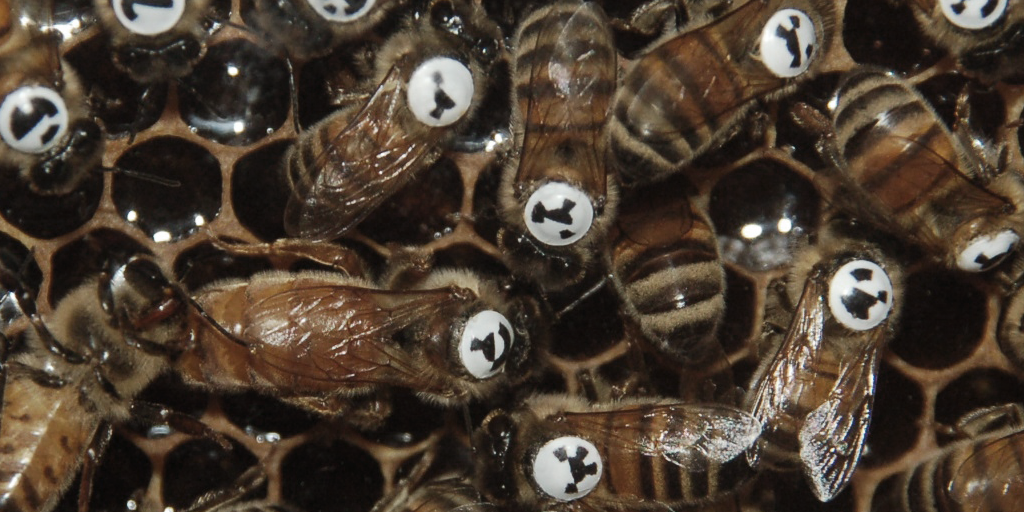
\includegraphics[width=1.0\textwidth]{Figures/markers}
	\caption{Tagged bees inside the hive.}
	\label{fig:markers}
\end{figure}

\section{Motivation}

Most of the studies analysing behaviour of insects colonies only use a small amount of individually labeled animals, a short observation period, and usually manually detect interaction between animals looking at the videos. data~\cite{quevillon2015social}[TODO: more references]. Here it is done in a more inclusive way, all animals, long term observation, automatic detection of individuals.

\section{Research Goal}

The aim of this thesis is to investigate whether the provided data set of tracked honey bees is useful for creating worker-worker interaction networks using spatial proximity as a proxy for interactions between bees. Thus, I need to implement a pipeline to infer networks out of the data set. Furthermore I want to find out if the resulting networks are suitable for social network analysis.

I want to achive my research goal by answering the following questions:

\begin{enumerate}
\item \emph{Is it possible to infer networks with the provided data set?}\\
What challenges and limitations does the data set imply?
\item \emph{What kind of networks emerge and what are their properties?}\\
How are those networks characterized in and are they different from a random network?
\item \emph{Do community structures exists?}\\
Are those communities robust?
\item \emph{How are those communities characterized?}\\
Do they reflect known colony behaviour in terms of age and spatial distribution?
\item \emph{How do the communities evolve over time?}\\
Are they stabel over time and how do members change communities over time?

\end{enumerate}


\section{Methodology}

Network Science Approach.

\section{Outline}
[TODO]